\documentclass[a4j]{jarticle}
    \usepackage[dvipdfmx]{graphicx}
    \usepackage[ top=25truemm,bottom=37truemm,left=25truemm,right=25truemm]
    {geometry}
    \usepackage{ascmac}
    \usepackage{amsmath}
    \usepackage{array}
    \usepackage{here}
    \usepackage{url}
    \usepackage{listings, jlisting}
    \usepackage{cases}
    \usepackage{txfonts}
    \usepackage[subrefformat=parens]{subcaption}
    \renewcommand{\lstlistingname}{リスト}
\lstset{language=c,
  basicstyle=\ttfamily\scriptsize,
  commentstyle=\textit,
  classoffset=1,
  keywordstyle=\bfseries,
  frame=tRBl,
  framesep=5pt,
  showstringspaces=false,
  numbers=left,
  stepnumber=1,
  numberstyle=\tiny,
  tabsize=4
}

\makeatletter
\def\@thesis{ネットワークプログラミング2}
\def\id#1{\def\@id{#1}}
\def\department#1{\def\@department{#1}}

\def\@maketitle{
\begin{center}
{\huge \@thesis \par} %修士論文と記載される部分
\vspace{10mm}
{\LARGE\bf \@title \par}% 論文のタイトル部分
\vspace{10mm}
{\Large \@date\par}	% 提出年月日部分
\vspace{20mm}
{\Large \@department \par}	% 所属部分
{\Large 学籍番号 \@id \par}	% 学籍番号部分
\vspace{10mm}
{\Large 氏名 \@author}% 氏名 
\end{center}
\par\vskip 1.5em
}

\title{自由課題}
\date{提出日 2021年7月27日 14:20}
\department{組番号 409}
\id{17406}
\author{金澤雄大}

    \begin{document}
    \maketitle
    \thispagestyle{empty}
    \clearpage
    \addtocounter{page}{-1}
    \section{目的}
    ネットワークプログラミング2で学習した内容への理解を深めるために自由課題として製作物を作成することを目的とする.

    \section{製作物の説明}
    本章では製作物の説明として, 製作物の概要, 花札の基礎と用語, こいこいのルールの3つについて述べる.
    \subsection{製作物の概要}
    製作物として同期通信を利用して, 花札で遊べるゲームの1つである「こいこい」を作成した. こいこいは2人または3人で同じ絵柄の札を揃えて役を作るカードゲームで, ここでは2人での対局を想定している.
    また実装したこいこいのルールは任天堂のルール !文献 を参考に, 一部プログラミングがしやすいように改変した.

    \subsection{花札の基礎と用語}
    花札の基礎と用語について説明する. 花札のカードは全48枚の札から構成されている. 札には1月から12月までの札が各4枚ずつ存在する. 各月の札の絵柄は図\ref{jan}~図\ref{dec}に示す通りである.
    札は月とは別に描かれている絵の種類で光札, タネ札, タン札, カス札の4種類に分けられる. 光札は最もレア度の高い札で1月の鶴が描かれている札, 3月の桜と幕が描かれている札, 8月の月が描かれている札, 11月の小野道風にカエル
    が描かれている札, 12月の桐に鳳凰が描かれている札の5枚のみである. タネ札は光札以外で動物や橋, 盃(さかずき)が描かれている札である. タン札は短冊が描かれている札である. カス札は植物のみが描かれている札である. 間違えやすい
    札として11月のカス札がある. 11月のカス札は黒と赤で構成されていて, 太鼓のようなものが描かれているがカス札である. 例外として9月のタネ札(盃が描かれている札)はタン札とタネ札の両方としてカウントする.
    
    \begin{figure}[H]
    \centering
    
\includegraphics[scale=1.5]{./img/jan.eps}
    \caption{1月 松に鶴}
    \label{jan}
    \end{figure}

    \begin{figure}[H]
    \centering
    
\includegraphics[scale=1.5]{./img/feb.eps}
    \caption{2月 梅にうぐいす}
    \label{feb}
    \end{figure}

    \begin{figure}[H]
    \centering
    
\includegraphics[scale=1.5]{./img/mar.eps}
    \caption{3月 桜に幕}
    \label{mar}
    \end{figure}

    \begin{figure}[H]
      \centering
      
\includegraphics[scale=1.5]{./img/apr.eps}
      \caption{4月 藤にほととぎす}
      \label{apr}
      \end{figure}
  
      \begin{figure}[H]
      \centering
      
\includegraphics[scale=1.5]{./img/may.eps}
      \caption{5月 菖蒲(アヤメ)に八ツ橋}
      \label{may}
      \end{figure}
  
      \begin{figure}[H]
      \centering
      
\includegraphics[scale=1.5]{./img/jun.eps}
      \caption{6月 牡丹に蝶}
      \label{jun}
    \end{figure}

    \begin{figure}[H]
      \centering
      
\includegraphics[scale=1.5]{./img/jul.eps}
      \caption{7月 萩に猪}
      \label{jul}
      \end{figure}
  
      \begin{figure}[H]
      \centering
      
\includegraphics[scale=1.5]{./img/aug.eps}
      \caption{8月 ススキに月・雁}
      \label{aug}
      \end{figure}
  
      \begin{figure}[H]
      \centering
      
\includegraphics[scale=1.5]{./img/sep.eps}
      \caption{9月 菊に盃(さかずき)}
      \label{sep}
      \end{figure}

    \begin{figure}[H]
      \centering
      
\includegraphics[scale=1.5]{./img/oct.eps}
      \caption{10月 紅葉に鹿}
      \label{oct}
      \end{figure}
  
      \begin{figure}[H]
      \centering
      
\includegraphics[scale=1.5]{./img/nov.eps}
      \caption{11月 小野道風にカエル, 柳にツバメ}
      \label{nov}
      \end{figure}
  
      \begin{figure}[H]
      \centering
      
\includegraphics[scale=1.5]{./img/dec.eps}
      \caption{12月 桐に鳳凰}
      \label{dec}
      \end{figure}

    \subsection{こいこいのルール}
      こいこいは花札を使用するゲームの1つである. 対局は2人または3人で行うが, ここでは2人で対局を行うときのルールについて説明する.
      こいこいは12回親と子を変えて対局し, 12回目の対局が終了したときに得点が高いほうが勝利するというルールである. \\
       対局手順について説明する. 1回目の対局では, はじめに親と子を決める. 親と子の決め方はまず, 48枚全ての札を裏返してシャッフルする. 次に親(先攻)と子(後攻)を決めるために, シャッフルした札から1枚ずつめくる. 
      めくった札の月が早いほうが親, 遅いほうが子である. 月が同じときは親子決めをやり直す. 親子が決まったら, 親が全ての札を裏返してシャッフルする. そして親が親, 子, 場にシャッフルした札を
      配る. 親と子は裏向き, 場は表向きで札を配る. 残った札は山札として裏向き重ねて置いておく. これで対局を始める準備ができた. また2回目以降の対局は親と子を交互に交代する. \\
       対局は親のターンから始まり, 親のターンが終わると子, 子のターンが終わると再び親のターンに戻る形式である. ターン中の行動は図\ref{turn-flow}のフローチャートの通りである.
      図\ref{turn-flow}の「こいこい」とはまだゲームを続けるかやめるかを選択することである. 「こいこい」を宣言すると相手のターンになり, 「あがり」を宣言すると対局が終了し, 
      こいこいを宣言した側の勝ちとなる. こいこいを宣言した後に相手の役(後述)ができると相手の役の得点が2倍になるためこいこいするかどうかは慎重に判断する必要がある.

      \begin{figure}[H]
      \centering
      \includegraphics[scale=1.8]{./img/turn-flow.eps}
      \caption{ターン中の行動手順}
      \label{turn-flow}
      \end{figure}

      役について説明する. 役とは手元に特定の札が揃ったときに自分の得点になり, こいこいするかどうかを決めるためのものである. 今回は次に示す11個の役を実装した. 
      ここに示す以外の役(例:手四, くっつき)もあるがここではそれらの役の判定は行わないものとする.
      \begin{itemize}
        \item 五光(10点) : 光札5枚が全て揃う.
        \item 四光(8点) : 11月の光札を除く光札4枚が揃う.
        \item 雨四光(7点) : 11月の光札とそれ以外の光札3枚が揃う.
        \item 三光(5点) : 11月の光札を除く光札3枚が揃う.
        \item 花見で一杯(5点) : 3月の光札, 9月のタネ札が揃う.
        \item 月見で一杯(5点) : 8月の光札, 9月のタネ札が揃う.
        \item 猪鹿蝶(5点) : 6月, 7月, 10月のタネ札3枚が揃う.
        \item 赤短(5点) : 1月, 2月, 3月のタン札3枚が揃う.
        \item 青短(5点) : 6月, 9月, 10月のタン札3枚が揃う.
        \item タネ : タネ札5枚で1点, 1枚増えるごとに1点追加.
        \item タン : タン札5枚で1点, 1枚増えるごとに1点追加.
        \item カス : カス札10枚で1点, 1枚増えるごとに1点追加.
      \end{itemize}
      

    \section{実行環境とビルド方法}
    本章では, 実行環境, ファイル構成, ビルド方法の3つについて述べる.
    \subsection{実行環境}
    表\ref{env}に実行環境を示す. OpenGLとGLpngは4年次にプログラミング演習で使用したものを用いる.  
    \begin{table}[H]
        \caption{実行環境}
      \label{env}
      \begin{center}
          \begin{tabular}{c|l}\hline
            CPU & Intel(R) Core(TM) i7-6500U 2.50GHz  \\ 
            メモリ & 16.0GB DDR4 \\
            OS & Microsoft Windows 10 Home \\
            gcc &  version 9.3.0 \\
            make & version 4.3 \\ \hline
          \end{tabular}
      \end{center}
      \end{table}

    \subsection{ファイル構成}
    リスト\ref{files}に製作したゲームのファイル構成を示す. 本ゲームはGoogle Drive!リンクでダウンロード
    できるようになっている. mylibディレクトリは授業中に作成したソケット通信用のライブラリである. 花札を実現するプログラムは
    mainディレクトリに入っている. さらにmainディレクトリ内にcardディレクトリがあり札の画像ファイルを格納している.
    \begin{lstlisting}[basicstyle=\ttfamily\footnotesize, frame=single,label=files,caption=ファイル構成]
5J_hanahuda
├── main
│   └── card
├── mylib
├── readme_img
└── readme.md
    \end{lstlisting}

    \subsection{ビルド方法}
ビルド方法について説明する. Google Driveからj17406.tar.gzをダウンロードして解凍した状態とする. まず, mylibディレクトリで
makeコマンドを実行してソケット通信用のプログラムをコンパイルする. 次にmainディレクトリでmakeコマンドを実行して花札を実行するプログラムをコンパイルする.
コンパイルができたら, s.exeとc.exeを実行すると対局が始まる.

    \section{プログラムの説明}
    本章ではserver.c, client.c, hanahuda.cの3つのプログラムの説明について述べる.
    \subsection{server.c}
    サーバー端末で動作するserver.cについて説明する. リスト\ref{server}にserver.cのプログラムを示す.
    リスト\ref{server}の10行目から28行目はOpenGLの処理である. 12行目から14行目ではウィンドウの生成を行っている.  
    16行目から21行目で動的な画面の描画, ウィンドウサイズの変更, キーボード, マウス処理のためにコールバック関数登録をしている.
    23行目から28行目ではアルファチャネルの有効化と背景色の変更の処理を行っている. 29行目から31行目では, サーバーのセットアップの処理
    を行っている. セットアップが失敗した場合は実行を終了する. 34行目では対局の初期化を行っている. game\_init関数の処理内容は
    4.3章のhanahuda.cで説明する. 最後に37行目でOpenGLのメインループに入る処理を行う. サンプルの五目並べのプログラムでは
    while文を用いたメインループでゲームの進行を行ったが, この処理をOpenGLに置き換えることでグラフィカルなゲームを実現している.
    \begin{lstlisting}[basicstyle=\ttfamily\footnotesize, frame=single,label=server,caption=server.c]
#include<stdio.h>
#include "hanahuda.h"
#include<GL/glut.h>
#include <GL/glpng.h>

int main(int argc,char **argv){
    int soc;
    // 初期化処理
    // 引数処理
    glutInit(&argc,argv);
    // 初期Windowサイズ設定
    glutInitWindowSize(WINDOW_W,WINDOW_H);
    // 新規Window作成
    glutCreateWindow("hanahuda_host");
    // 関数登録
    glutDisplayFunc(Display);
    glutReshapeFunc(Reshape);
    glutKeyboardFunc(Keyboard);
    glutMouseFunc(Mouse);
    glutPassiveMotionFunc(PassiveMotion);
    glutTimerFunc(500,Timer,0);
    //  テクスチャのアルファチャネルを有効にする設定
    glEnable(GL_BLEND);
    glBlendFunc(GL_SRC_ALPHA, GL_ONE_MINUS_SRC_ALPHA);
    glTexEnvf(GL_TEXTURE_ENV, GL_TEXTURE_ENV_MODE, GL_MODULATE);
    // display初期化
    glutInitDisplayMode(GLUT_RGBA);
    glClearColor(0.28,0.48,0.32,1.0);
    if( (soc=setup_server(PORT))==-1){
        exit(1);
    }

    // ゲーム初期化
    game_init(soc,0);

    // glutのメインループ
    glutMainLoop();
    return 0;
}
          \end{lstlisting}

    \subsection{client.c}
    クライアント端末で動作するclient.cについて説明する. client.cのプログラムをリスト\ref{client}に示す. 基本的な処理の流れはserver.cと同じである. 
    server.cとの違いは31行目から38行目である. 30行目および31行目では接続するホスト(サーバー)名を入力させる処理を行っている. ホスト名は「localhost」,「192.168.10.4」
    のように入力する. 33行目で実行しているchop\_newline関数はmylibディレクトリで定義されている関数で
    入力した文字列の末尾の改行文字をナル文字に置換する機能を持つ. 36行目から38行目では入力されたホストのIPアドレスをもとにクライアントのセットアップの処理を行っている.
    \begin{lstlisting}[basicstyle=\ttfamily\footnotesize, frame=single,label=client,caption=client.c]
#include<stdio.h>
#include "hanahuda.h"
#include<GL/glut.h>
#include <GL/glpng.h>

int main(int argc,char **argv){
    int soc;
    char hostname[64];
    // 初期化処理
    // 引数処理
    glutInit(&argc,argv);
    // 初期Windowサイズ設定
    glutInitWindowSize(WINDOW_W,WINDOW_H);
    // 新規Window作成
    glutCreateWindow("hanahuda_client");
    // 関数登録
    glutDisplayFunc(Display);
    glutReshapeFunc(Reshape);
    glutKeyboardFunc(Keyboard);
    glutMouseFunc(Mouse);
    glutPassiveMotionFunc(PassiveMotion);
    glutTimerFunc(500,Timer,0);
    //  テクスチャのアルファチャネルを有効にする設定
    glEnable(GL_BLEND);
    glBlendFunc(GL_SRC_ALPHA, GL_ONE_MINUS_SRC_ALPHA);
    glTexEnvf(GL_TEXTURE_ENV, GL_TEXTURE_ENV_MODE, GL_MODULATE);
    // display初期化
    glutInitDisplayMode(GLUT_RGBA);
    glClearColor(0.28,0.48,0.32,1.0);
    //サーバーのホスト名の入力
    printf("Input server's hostname: ");
    fgets(hostname,HOSTNAME_LENGTH,stdin);
    chop_newline(hostname,HOSTNAME_LENGTH);

    //接続完了まで
    if((soc = setup_client(hostname,PORT)) == -1){
        exit(1);
    }

    // ゲーム初期化
    game_init(soc,1);
    
    // glutのメインループ
    glutMainLoop();

    return 0;
}
          \end{lstlisting}

    \subsection{hanahuda.c}
    本節ではhanahuda.cにおける構造体および関数の説明について述べる.
    \subsubsection{札の処理}
    札の扱いと処理について説明する. 札はリスト\ref{cardstruct}に示すcard構造体の配列で定義されている. card構造体は
    月, 画像ファイルの番号, 札の種類の3つをメンバとして持っている.
    \begin{lstlisting}[basicstyle=\ttfamily\footnotesize, frame=single,label=cardstruct,caption=card構造体]
// 札用の構造体
struct cardstruct{
    int month; // 1-12
    int num; // imgの番号
    int rank; //1-4, 4:光札,3:タネ札,2:短冊札,1:カス札
};
typedef struct cardstruct card;
// 札用の構造体の配列を定義
static card cards[CARD_NUM];      
    \end{lstlisting}
    次に山札や場札から出すときの処理について説明する. 山札と手札は札を出す, 場札は札の出し入れの処理を行う必要がある.
    また獲得した札を保持する配列が必要である. これらの処理を行うために, javaにおけるsetterとgetterにあたる関数を用意した.
    リスト\ref{setget}に山札, 場札, 手札, 獲得した札の配列に札を出入力する関数を示す. 関数名がpopで始まる関数は札を管理する配列から
    札を取り出す関数, pushで始まるものは札を入力する関数である. 
    \begin{lstlisting}[basicstyle=\ttfamily\footnotesize, frame=single,label=setget,caption=札の入出力をする関数]
// 山札から札を出す処理
// 札のインデックスを返す
int popDeck(void){
    deck_num++;
    return deck[deck_num-1];
}

// 場に札を入れる処理
void pushPlace(int c){
    place[place_num++]=c;
}

// 場から札を出す処理
int popPlace(int index){
    int i;
    int tmp=place[index];
    for(i=index+1;i<place_num;i++){
        place[i-1]=place[i];
    }
    place[i-1]=-1;
    place_num--;
    return tmp;
}

// 手札から札を出す処理
int popHandCard(int index){
    int i;
    int tmp;
    if(role==0){ // 親のとき
        tmp = mycard[index];
        for(i=index+1;i<mycard_num;i++){
            mycard[i-1]=mycard[i];
        }
        mycard[mycard_num-1]=-1;
        mycard_num--;
    }else{ // 子のとき
        tmp = peercard[index];
        for(i=index+1;i<peercard_num;i++){
            peercard[i-1]=peercard[i];
        }
        peercard[peercard_num-1]=-1;
        peercard_num--;        
    }
    return tmp;    
}

// 持ち札に札を入れる処理
void pushgetCard(int c){
    if(role==0){
        mygetcard[mygetcard_num]=c;
        mygetcard_num++;
    }else{
        peergetcard[peergetcard_num]=c;
        peergetcard_num++;
    }
} 
    \end{lstlisting}

    \subsubsection{ゲームの初期化処理}
    ゲームの初期化処理について説明する. ゲームの初期化はリスト\ref{initgame}の3行目から15行目に示すgame\_init関数を実行することで行われる.
    game\_init関数の内部では, まず6行目で親と子の区別をするための変数roleに引数から受け取った値を代入する処理を行っている. 親のときリスト\ref{server}の34行目に示したように, 
    roleを0, 子のときリスト\ref{client}の41行目で示したようにroleを1に設定している. \\
     8行目では配列の初期化を行う関数であるarray\_init関数を実行している. array\_init関数の定義は44行目から46行目である. 9行目ではreadImg関数を実行している.
    readImg関数の定義は18行目から41行目である. readImg関数ではcardディレクトリに置いたある札の画像を取得しcardimg配列に代入する処理を行っている. カード名をsprintf関数で指定してから
    指定されたパスの画像を取得するpngBind関数を実行することで48枚の札の取得を実現している.\\
     11行目から14行目では山札をシャッフルして場と手札に札を配る処理を行っている. 山札のシャッフルは83行目から100行目に定義したshuffle関数で行っている. 花札の札には重複がないため乱数をランダムに代入して
    山札を生成することができない. そこで0から47までの数字が1つずつ入った配列を生成し, ランダムに2つを選択して交換する処理を何度か繰り返すことで重複のないランダムなリストを生成している.
    交換回数は10000回としている. 山札の設定が終わったから104行目から127行目に示すarrangeCard関数を用いて場と2人の手札にそれぞれ8まいずつ札を配る処理を行っている. このとき, 場に3枚以上同じ月の札がでたら
    山札のシャッフルと札の分配をやり直すかどうかの判定を行い, やり直しの必要があるときは1を返すようにしている. game\_init関数関数では返り値が0になるまでループさせることで
    場に取れない札がでることを防止している. なお本来の対局では場に3枚同じ札が出た時は残りの1枚を場に出したときに4枚すべて獲得できる, または場に出ている3枚から1枚をランダムに山札に戻して別の1枚をだし, 山札をシャッフルしなおすという
    ルールになっている. 場に4枚同じ札がでたときのルールは公式なものはないが場と山札をシャッフルしなおすのが一般的であると考える.
    \begin{lstlisting}[basicstyle=\ttfamily\footnotesize, frame=single,label=initgame,caption=ゲームの初期化処理]
// 対局初期化
// role 0:親,1:子
void game_init(int soc,int argrole){
    int tmp=1;
    hanahuda_soc = soc;
    role=argrole;
    
    array_init();
    readImg(); // 画像読み込み
    card_init(); // 札情報をcardstruct構造体に格納
    while(tmp==1){
        shuffle(); // 山札シャッフル
        tmp=arrangeCard(); // 場, 手札に札を配る
    }
}

// 画像読み込み
void readImg(void){
    char fname[100];
    int i,j;
    int cnt=0;
    // 全札読み込み
    for(i=0;i<MONTH;i++){
        for(j=0;j<MONTH_CARD;j++){
            sprintf(fname,".\\card\\%s-%d.png",month[i],j+1);
            //printf("%s\n",fname);
            cardimg[cnt] = pngBind(fname, PNG_NOMIPMAP, PNG_ALPHA, 
                &cardinfo[cnt], GL_CLAMP, GL_NEAREST, GL_NEAREST);
            cnt++;
        }
    }
    // 裏返しの黒い札(back)を読み込み
    sprintf(fname,".\\card\\back.png");
    cardimg[cnt] = pngBind(fname, PNG_NOMIPMAP, PNG_ALPHA, 
        &cardinfo[cnt], GL_CLAMP, GL_NEAREST, GL_NEAREST);

    // こいこい時のポップアップ用の画像を読み込む処理
    sprintf(fname,".\\koikoi.png");
    koikoiimg = pngBind(fname, PNG_NOMIPMAP, PNG_ALPHA, 
        &koikoiinfo, GL_CLAMP, GL_NEAREST, GL_NEAREST);        
}

// 配列の初期化
void array_init(void){
    int i;
    // 配列の初期化
    for(i=0;i<PLACE_MAX;i++){
        place[i]=-1;
    }
    for(i=0;i<INIT_PLACE;i++){
        mycard[i]=-1;
        peercard[i]=-1;
    }
    for(i=0;i<CARD_NUM/2;i++){
        mygetcard[i]=-1;
        peergetcard[i]=-1;
    }
    for(i=0;i<PLACE_MAX;i++){
        place[i]=-1;
    }
    for(i=0;i<YAKU_NUM;i++){
        myyaku[i]=0;
        peeryaku[i]=0;
    }    
}

// 札の情報をカード構造体に格納
void card_init(void){
    int i,j;
    int cnt=0;
    // すべての札について
    for(i=1;i<=MONTH;i++){ // 12回(月の回数)ループ
        for(j=0;j<MONTH_CARD;j++){ // 4回ループ
            cards[cnt].month=i; // 月
            cards[cnt].num=j+1; // 札番号
            cards[cnt].rank=cardrank[i-1][j]; // 点数
            cnt++;
        }
    }
}

// 札をシャッフル
void shuffle(void){

    int i,rnd1,rnd2,tmp;
    srand((unsigned) time(NULL)); // 乱数初期化
    // 全ての札を山札に格納
    for(i=0;i<CARD_NUM;i++){
        deck[i]=i;
    }

    for(i=0;i<SHUFFLE_TIME;i++){
        rnd1 = rand()%CARD_NUM; // ランダムに1枚指定
        rnd2 = rand()%CARD_NUM; // ランダムに1枚指定
        // 指定した札を交換
        tmp = deck[rnd1];
        deck[rnd1] = deck[rnd2];
        deck[rnd2]=tmp;
    }
}

// 場と手札に札を配る処理
// 場札に同じ月の札が3枚以上あるとき1,それ以外のとき0を返す.
int  arrangeCard(void){
    int i,j,tmp;
    // 場,親,子に8枚札を出す
    for(i=0;i<INIT_PLACE;i++){
        pushPlace(popDeck());
        mycard[i] = popDeck();
        peercard[i] = popDeck();
    }
        // 場の状態を確認
    for(i=1;i<=MONTH;i++){
        tmp=0;
        for(j=0;j<place_num;j++){
            if(cards[place[j]].month==i){
                tmp++;
            }
        }
        if(tmp>=3){ // 場に3枚以上同じ月の札があるとき
            tmp=1;
            return tmp;
        }
    }
    tmp=0;
    return tmp;
}
    \end{lstlisting}

    \subsubsection{画面描画の処理}
    画面描画処理について説明する. 画面描画処理が行われるタイミングはウィンドウサイズが変更されたとき, タイマーによってウィンドウの再描画
    関数が実行されたときの2つである. ウィンドウサイズが変更されるとリスト\ref{reshape}に示すReshape関数がコールバック関数として実行される. 
    Reshape関数が実行されると, ウィンドウの再生成が行われるが, このゲームでウィンドウサイズが自由に変えられると困るため10行目のglutReshapeWindow関数で
    ウィンドウサイズを600x600に固定している.
\begin{lstlisting}[basicstyle=\ttfamily\footnotesize, frame=single,label=reshape,caption=Reshape関数]
void Reshape(int w,int h){
    glViewport(0,0,w,h);
    glMatrixMode(GL_MODELVIEW);
    glLoadIdentity();
    gluOrtho2D(0,w,0,h);
    glScaled(1,-1,1);
    glTranslated(0,-h,0);

    //windowサイズ固定 
    glutReshapeWindow(WINDOW_W,WINDOW_H);
}
\end{lstlisting}
  タイマーによってウィンドウの再描画関数が実行されたとき, リスト\ref{timer}に示すTimer関数が実行され, Timer関数がDisplay関数を呼び出す.
  Display関数はゲーム全体の流れを  

    \subsubsection{マウス, キーボードの入力処理}
    \subsubsection{役の処理}
    \subsubsection{ゲームの進行処理}

    \subsection{hanahuda.h}
    リスト\ref{hanahudah}にhanahuda.hのコードを示す.
    \begin{lstlisting}[basicstyle=\ttfamily\footnotesize, frame=single,label=hanahudah,caption=hanahuda.h]
    \end{lstlisting}

        \begin{thebibliography}{9}
          \bibitem{NNCT}  国立高専機構長野高専,\url{http://www.nagano-nct.ac.jp/} ,閲覧日2020年8月5日
          \end{thebibliography}
\end{document}

